\documentclass[conference]{IEEEtran}
% If IEEEtran.cls has not been installed into the LaTeX system files,
% manually specify the path to it like:
% \documentclass[conference]{../sty/IEEEtran}
\usepackage[english]{babel} 
\usepackage{longtable}
\usepackage{ifpdf}
\usepackage[table]{xcolor}

\usepackage{anysize}
\usepackage{textcomp}
\usepackage{url}
\bibliographystyle{unsrt}
\usepackage{graphics}
\usepackage{amssymb}
\usepackage{graphicx}
%\usepackage{slashbox}
\usepackage[latin1]{inputenc}
\usepackage{tikz}
\usetikzlibrary{shapes.geometric, positioning, calc}
\usepackage{pgfplots}
\usepackage{amsmath}
\usepackage{float}
\usetikzlibrary{arrows,positioning,patterns}
% Color and strikethrough
\usepackage{color}
\usepackage{soul}

\usepackage{array}
\usepackage{makecell}
\usepackage{multirow}
\usepackage{caption}

\usepackage[]{algorithm2e}

\usepackage{cite}
\usepackage{tabu}
\usepackage{caption}
\captionsetup[table]{skip=1pt}
\usepackage{paralist}
\usepackage[a4paper, total={7in, 9in}]{geometry}


%\usepackage{sectsty}
% correct bad hyphenation here
\hyphenation{op-tical net-works semi-conduc-tor}


\begin{document}
 \graphicspath{{./}{./fig/}}
%
% paper title
% Titles are generally capitalized except for words such as a, an, and, as,
% at, but, by, for, in, nor, of, on, or, the, to and up, which are usually
% not capitalized unless they are the first or last word of the title.
% Linebreaks \\ can be used within to get better formatting as desired.
% Do not put math or special symbols in the title.
\title{Towards using of ASIPs for Approximate Computing}


% author names and affiliations
% use a multiple column layout for up to three different
% affiliations
\author{\IEEEauthorblockN{Daniel Moya S\'anchez}
\IEEEauthorblockA{Computer Engineering Academic Area\\
Instituto Tecnol\'ogico de Costa Rica\\
Email: danielmscr1994@gmail.com}}

% make the title area
\maketitle

% As a general rule, do not put math, special symbols or citations
% in the abstract
\begin{abstract}
IT systems have been facing challenges such as cost in area, power. and execution time, which restrict 
the performance of a chip.  Approximate computing is a novel design paradigm that proposes a 
reduction in the accuracy or precision of computations to find opportunities for improvement in terms 
of area, power, and execution time. This paper evaluates the design of Application-Specific Instruction 
Processors (ASIPs) for error-tolerant applications in three specific applications, through the use of 
ASIPMeister and Dlxsim tools, which allow the synthesis required for a processor's hardware with its 
Instruction Set Architecture (ISA). Speedups in the total cycles were achieved from 1.08X to 1.91X, 
while adding minimal area (1\% at most) and power (maximun of 5 mW) requirements.


%NOTA: el abstract lo terminamos de definir/pulir una vez que el paper este listo
\end{abstract}


\IEEEpeerreviewmaketitle



\section{Introduction}

Information Technology (IT) systems seek to give a better quality of
life to people. In this task, these systems have been facing
certain challenges, among them the cost in area, power, and execution time, which
restrict the performance of a chip. Ideally, an application should fit the
real needs of the user and, in general, of the area of application, so that an optimal
use of resources is achieved. Currently, processor design is not only focused on
having more performance but also an appropriate resource management;
however, some challenges in this field are due to physical limitations,
for instance:

\begin{compactitem}
 \item electrical characteristics of the CMOS transistors, which
 restrict the energy consumption in embedded systems and which is an issue
 that designers should consider for specific purpose
 components in processors;
 
 \item memory wall, which corresponds to the difference between the growth
 of processing capacity against the speed of data gathering
 from memory;

 \item and utilization wall, which limits the maximum use of hardware
 simultaneously due to the heat dissipation capability of a system.
\end{compactitem}

In order to face the problems mentioned above, a current research area corresponds to 
approximate computing. This is a novel
design paradigm that proposes a reduction in the accuracy or precision of
computations to obtain opportunities for improvement in
area, power and execution time. To apply this paradigm, it is necessary to
identify error-tolerant applications and determine, in a specific manner,
which sections or functions within these can be replaced by
approximate versions, so that a balance can be obtained between the output quality
 and the general computing resources required. For a given error-tolerant system, 
 the framework on Figure \ref{fig:ap} can be applied to 
include the approximate computing paradigm \cite{xu2018approximate}.

%NOTA: Podrias mencionar los diferentes niveles de abstraccion a los cuales se ha 
%utilizado AC. Adem�s, el salto a ASIPs se da de manera abrupta en el siguiente p�rrafo y 
%no queda un enlance entre lo que venis contando. Adem�s, el resumen de la contribuci�n, 
%que a este punto vas a aclarar, debe ser consecuente con lo que finalmente va a 
%presentarse en el documento.


\begin{figure}
\begin{center}
 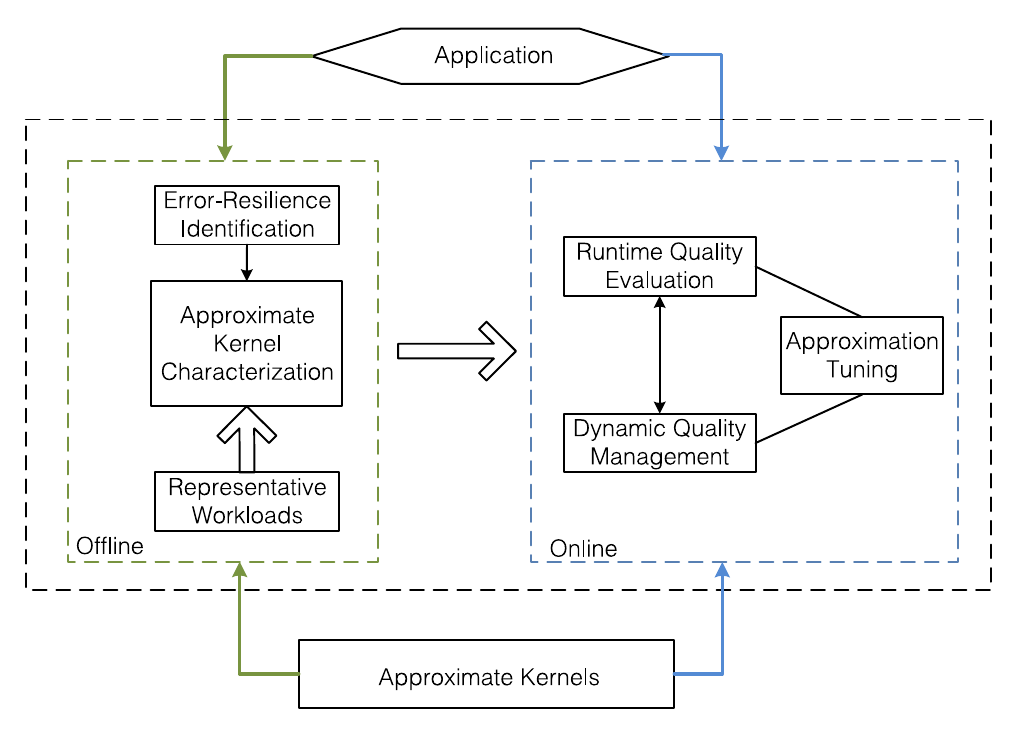
\includegraphics[width=0.5\textwidth]{APframework}
 \caption{An existing approximate computing framework. Taken from \cite{xu2018approximate}} \label{fig:ap}
 \end{center}
\end{figure}

The key elements of Figure \ref{fig:ap} consist of approximate kernels, which are
the implementation (techniques) of the approximate functions, these could be done at a hardware layer or at
a software layer; the identification of the error-tolerant parts
and its specific details (e.g. impact analysis); and the quality management which implies a continuos evaluation to determine
if the application meets the desired requirements \cite{xu2018approximate}.

One way to implement approximate computing is through Application-Specific Instruction 
Processors (ASIPs). An ASIP is a processor that uses an application-specific instruction 
set, this means 
that, although it can execute a wide range of applications, it is optimized for a 
specific one, in which the ASIP can execute with improved performance (for instance, 
energy consumption or execution time would be lower) compared to a General Purpose Proccesor (GPP).
With the use of ASIPs, instructions and even functions where there is error tolerance can be
implemented as special approximated instructions, that reduce the resource consumption 
while keeping the error from the approximation under an acceptable threshold. Although Application Specific Integrated Circuits (ASICs) show better performance 
results, ASIPs possess more flexibility. Optimizations for an ASIP can be seen in different forms, 
including \cite{henkel2003closing}:

\begin{itemize}
 \item Instruction extension: Customized instructions can be made to extend the base Instruction Set Architecture (ISA).
 
 \item Inclusion or exclusion of predefined blocks: Not only specific software can be added 
 to extend an architecture but also customized hardware in the form of specialized blocks; 
 also, regular blocks not used can be excluded.
 
 \item Parameterization: Certain variables, such as cache sizes or number of registers, can 
 be customized to adjust for a specific application.
\end{itemize}

ASICs represent a hardware solution to a problem which is very limited and have high 
costs and a high time-to-market, but achieve the greatest performance. Contrary, GPPs 
are seen as a software solution which are very flexible but they are the least efficient. ASIPs
are in the middle of these two as they balance flexibility and performance to have a 
good trade-off between those variables. 

\vspace{6pt}
\noindent
\textbf{Contribution: }
This work evaluates the design performance, in area, power, and execution time, of ASIPs with special 
instructions
for error-tolerant applications. For this purpose, three different error-tolerant applications
were evaluated and then, for each one, an special instruction, that reflects a recurrent operation 
in the original code, was implemented. Finally, the performance of each optimization
was evaluated against the original version to determine the impact of the designed ASIPs.

Since translating a whole application from the C programming language to assembly
code was too costly, only a smaller version which contains the key processing
was developed for testing purposes. The ASIPs developed do not use explicitly 
approximate hardware, this is considered the main future work for this paper.


%NOTA: Una vez que el resto de las secciones est�n completas, hay que iterarar 
%nuevamente la introducci�n para que todo sea consecuente.

\section{Context and background}

% In the current era, where sophisticated applications are widely used (e.g. GPS systems, 
% speech recognition, etc.) approximate computing helps delivering acceptable
% output while keeping metrics such as response time or energy efficiency at better levels. 
% Approximate computing gives the freedom to tradeoff certain error level or allow quality degradation in the final output
% of an application (e.g. noise in the output signal) for lower energy consumption, area or execution time, thus
% giving the researcher a tool to adjust with the real and specific needs of a given application.

% For a given error-tolerant system, the framework on figure \ref{fig:ap} can be applied to 
% include the approximate computing paradigm \cite{xu2018approximate}.

%NOTA: el contenido de este p�rrafo se puede usar para la introducci�n y no ac�. La 
%idea de esta secci�n es que sea un Related Work y, como te coment� el otro d�a, te 
%enfoques en contar algunas tecnicas de computaci�n aproximada que se han aplicado a 
%GPPs y otras a ASICs (ver lista que te envio al respecto), y por ah� dejar la puerta abierta 
%para mencionar que a�n no se ha hecho mucho (o nada) a nivel de ASIPs


The relationship between GPPs, ASIPs, and ASICs is shown in Figure \ref{fig:gaa}.
Approximate computing techniques can also be implemented on GPPs, due to their 
extremely flexible nature.
However, because they are designed for any kind of computation, it falls on the 
programmers, or compilers, not on specialized hardware modules,
to make the performance of software running on these systems as high as possible. On the other hand, since ASICs are a pure hardware solution,
approximate hardware modules would be difficult to manage in terms of quality evaluation,
this could cause high cost of development, since the hardware would not be programmable. ASIPs can adjust to specific requirements of
a given application (through extended instructions) so that a better balance of cost savings and 
amount of error is achieved. This project focuses on that goal; to design ASIPs for a set 
of error-tolerant applications.


\begin{figure}
\begin{center}
 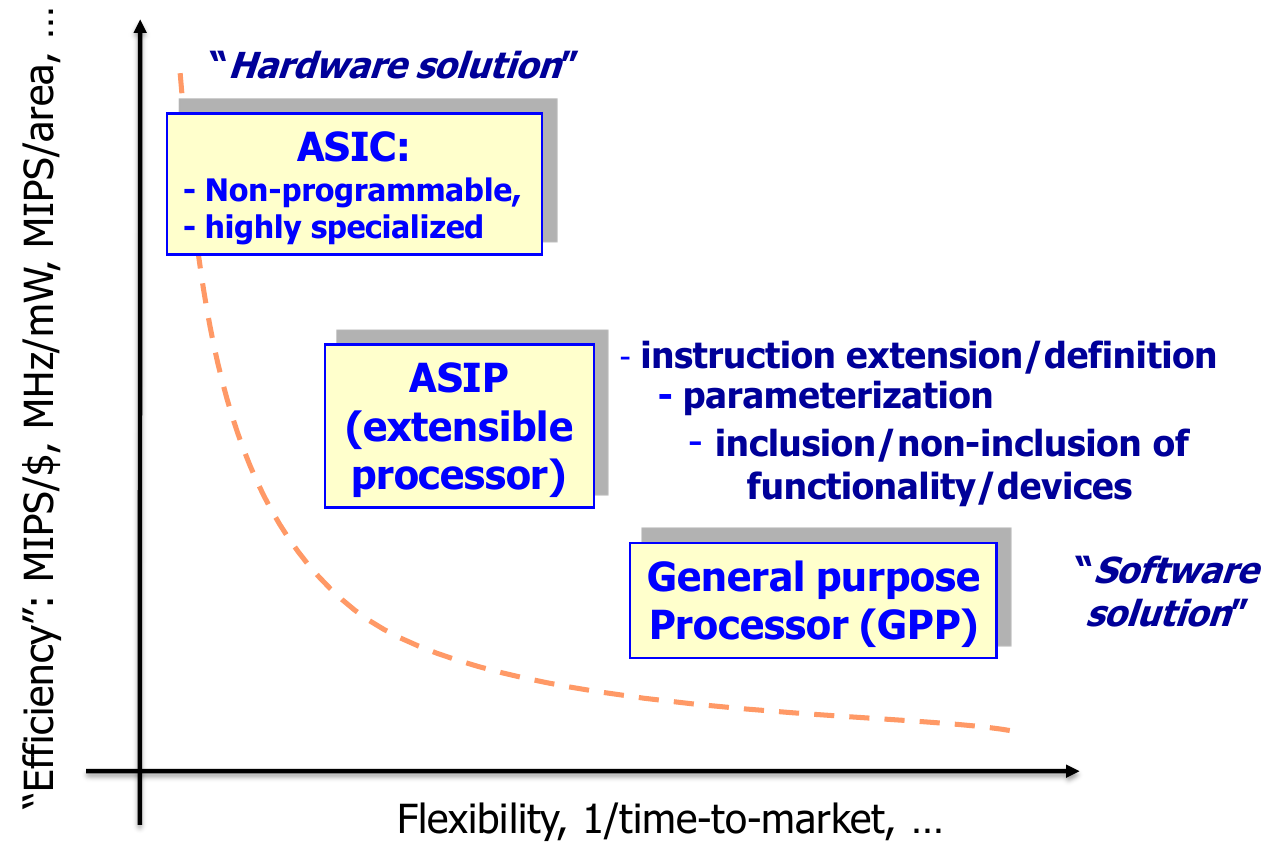
\includegraphics[width=0.5\textwidth]{GPP-ASIP-ASIC}
 \caption{Comparison between GPPs, ASIPs, and ASICs. Taken from \cite{henkel2006design}} \label{fig:gaa}
 \end{center}
\end{figure}



Some of the research efforts in the approximate computing area focus on software solutions, for example, in \cite{sidiroglou2011managing} the loop perforation technique
is explained, which uses two particular methods, criticality testing (filtering of critical loops) and perforation space exploration (determining the
best performance for a specific accuracy loss bound). A higher level solution is mentioned in \cite{tan2015approximation}, where a scheduling
framework for meeting the performance and thermal design power is proposed. Several versions of a task are used by the scheduler to provide
tradeoffs between different levels of quality of service and performance. A neural network based solution is detailed in \cite{esmaeilzadeh2013neural},
where a learning model is trained to identify how an approximable region of code behaves for different approximate versions.

On the other hand, hardware solutions have also been proposed; from approximate adders and multipliers to
the design of ASICs. For example, in \cite{venkataramani2012salsa} a methodology for the automation of creating approximate circuits is proposed.
The general idea involves using the original circuit as an input and a quality function to adjust and verify an approximate
circuit so the quality constraint is met for a given hardware configuration. A similar approach is taken in \cite{ranjan2014aslan}, where
contrary to the previous proposal, the approximate circuits are sequential, which extends the same purpose for more possible approximate
circuits. Finally, in \cite{nepal2014abacus}, a more global approach is taken, where the approximate circuits are generated using
behavioral-level descriptions (and not RTL like the previous proposals); from there, an Abstract Synthesis Tree (AST) is created,
which is later analyzed and modified to include the approximate circuit logic, so that, as the other methods, the circuit is tested and
its performance evaluated. 


\section{Design of the ASIPs}


As explained before, an ASIP is able to execute a wide range of operations but also some specialized instructions
for an specific application. Following this scheme, a general processor with common instructions (for example add,
substract, shift, among others) was used within the ASIPMeister tool, and one specific instruction was added for each different selected application.
This is showed in Figure \ref{fig:hardware}, where, for certain operations (controlled by the processor signals) the 
ALU is ignored and instead the result from the special additional hardware is used (Special 
Instruction, SI). 

\begin{figure}[t!]
\centering
\resizebox{0.5\textwidth}{!}{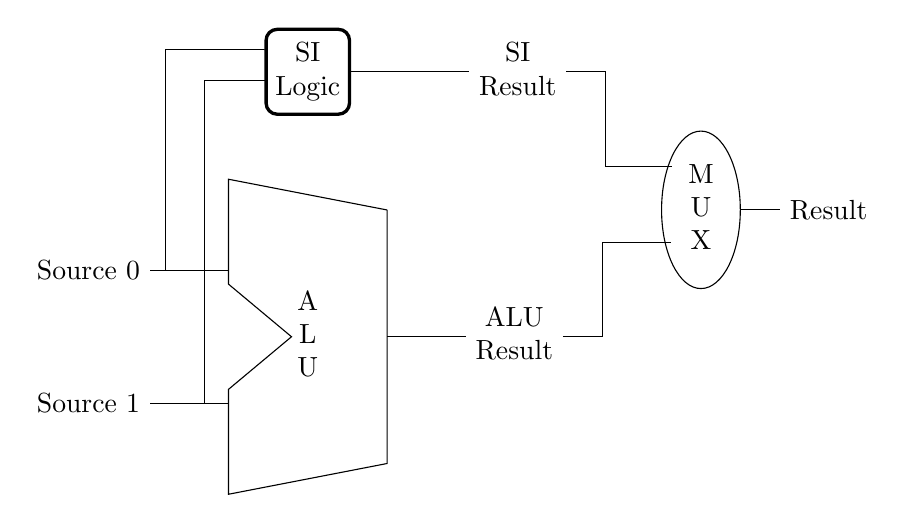
\begin{tikzpicture}[%
    alu/.style={trapezium,
            trapezium angle=70,
            shape border rotate=270,
            minimum width=4cm,
            minimum height=2cm,
            trapezium stretches=true,
            append after command={%
                    \pgfextra
                        \draw (\tikzlastnode.top left corner) --
                           (\tikzlastnode.top right corner) -- 
                           (\tikzlastnode.bottom right corner) -- 
                           ($(\tikzlastnode.bottom right corner)!.666!(\tikzlastnode.bottom side)$)--
                           ([xshift=8mm]\tikzlastnode.bottom side)--
                           ($(\tikzlastnode.bottom side)!.334!(\tikzlastnode.bottom left corner)$)--
                           (\tikzlastnode.bottom left corner)--
                           (\tikzlastnode.top left corner);
                    \endpgfextra}},
            ]

\node[alu] (alu) {\makecell{A\\L\\U}};
\draw (alu.east) -- ++(0:10mm) node [right] (aluResult) {\makecell{ALU\\Result}};
\draw (alu.220) -- ++(180:10mm) node [left] {Source 1};
\draw (alu.140) -- ++(180:10mm) node [left] {Source 0};

\node[rectangle, rounded corners,draw=black, very thick, minimum size=3em, above = 1cm 
of alu] (asip) {\makecell{SI\\Logic}};

\draw (alu.220) -- ++(180:3mm) -- ++(90:41mm)  -|  (asip.191);
\draw (alu.140) -- ++(180:8mm) -- ++(90:28mm)  -|  (asip.153);

\draw (asip.east) -- ++(0:15mm) node [right] (asipResult) {\makecell{SI\\Result}};

\draw (alu.122) ++(0:60mm) ellipse (5mm and 10mm) node (mux) {\makecell{M\\U\\X}};

\draw (aluResult.east) -- ++(0:5mm) -- ++(90:12mm) -- ++(0:8.7mm);
\draw (asipResult.east) -- ++(0:5mm) -- ++(270:12mm) -- ++(0:8.4mm);

\draw (mux.east) ++(0:2.2mm) -- ++(0:5mm) node [right] {Result};
\end{tikzpicture}}
\medskip
\caption{ASIP Hardware implentation.} 
\label{fig:hardware}
\end{figure}



The three aproximate applications found were K-Means, K-Nearest Neighbors (KNN) and the Sobel filter. 
All the special instructions correspond to new assembly instructions of arithmetic tpye, which modify the Instruction Set Architecture (ISA) using the Dlxsim tool. For the K-Means
application, the special instruction \emph{eucl} was implemented, which executes part of the euclidean distance operation,
as follows (considering \emph{rd} as the destination register, \emph{rs0} and \emph{rs1} as the registers with the input values):

\begin{align}
 rd = (rs0 - rs1)^2
\end{align}

At a hardware level, this instruction uses a combinatorial block (the ALU is not used), consisting in an adder (which executes a substraction when the second input
is negated) and a multiplier. At a software level, the \emph{eucl} instruction is used in the inner loop as the main operation in the calculation of the array index of the nearest cluster
center, as showed in the Algorithm \ref{algo:kmeans}.

\begin{algorithm}[h!]
\SetKwData{Left}{left}\SetKwData{This}{this}\SetKwData{Up}{up}
\SetKwFunction{Union}{Union}\SetKwFunction{FindCompress}{FindCompress}
\SetKwInOut{Input}{input}\SetKwInOut{Output}{output}
 \Input{Clusters, Number of clusters and coordinates}
 \Output{Array index of nearest cluster center}
\BlankLine

% \For{$k\leftarrow 1$ \KwTo number of objects}{
  $min\_dist\leftarrow \text{eucl$\_$distance}(num\_dims,coord1[0],coord2[0])$\;
  \For{$j\leftarrow 1$ \KwTo number of clusters}{
    \For{$i\leftarrow 1$ \KwTo of number of coordinates}{
    $dist \mathrel{+}= eucl(coord1[i],coord2[i])$\;
    }
  \If{$dist < min\_dist$}{$\newline min\_dist \leftarrow dist \newline index \leftarrow i$}
  }
  Return $i$ \medskip
%}
\caption{K-Means algorithm extract} \label{algo:kmeans}
\end{algorithm}


For the KNN application, the special instruction \emph{absv} was implemented, which executes a subtract operation with an absolute result, 
which is used frequently in the KNN algorithm (the euclidean distance remains the main operation in this algorithm too). At at high abstraction level,
this operation executes:

\begin{align}
 rd = rs0 > rs1 \,?\, rs0-rs1 : rs0-rs1
\end{align}
At a hardware level, a simple adder (which executes a substraction) and a mux are used, in an additional combinatorial block. At a software
level, the \emph{absv} instruction is used to compare the resulting estimate vs the actual prediction given by the user, where if 
the given prediction is within the 20\% of the resulting estimate, the prediction is considered correct, otherwise wrong, as showed
in the Algorithm \ref{algo:knn}.

\begin{algorithm}[h!]
\SetKwData{Left}{left}\SetKwData{This}{this}\SetKwData{Up}{up}
\SetKwFunction{Union}{Union}\SetKwFunction{FindCompress}{FindCompress}
\SetKwInOut{Input}{input}\SetKwInOut{Output}{output}
 \Input{Prediction attribute and k value}
 \Output{Number of correct predictions}
\BlankLine

  \For{$j\leftarrow 1$ \KwTo number of samples}{
  $N = \textit{number of validated samples}$\;
  $actual\leftarrow sample[N].Attributes[Predict\_attr]$\;
  $result\leftarrow \text{KNN}(N,k_value)$\;
  \If{$absv(actual,result)/actual < 0.2$}{$correct\_count++$}
  }
  Return $correct\_count$ \medskip
\caption{KNN algorithm extract} \label{algo:knn}
\end{algorithm}


For the last application, the Sobel filter, the special instruction \emph{sob} was developed, which allows computing the following operation in a single cycle:

 \begin{align}
  rd = rs0^2 + rs1^2
 \end{align}

The operation described in (3) allows the execution of two multiplications and an addition operation, which is used frequently in the Sobel algorithm. Other operations 
in this algorithm could not be turned into special instructions (for example, a matrix multiplication) because they require more than two paremeters. 

At a hardware level, this instruction requires two multipliers and one adder (the ALU is not used). At a software level, the \emph{sob} instruction is used
to weight the values from the convolution in both $x$ with $y$ dimensions, the result is used if it is not above a maximum threshold
(otherwise the maximum value is used), as showed in Algorithm \ref{algo:sobel}.

\begin{algorithm}[h!]
\SetKwData{Left}{left}\SetKwData{This}{this}\SetKwData{Up}{up}
\SetKwFunction{Union}{Union}\SetKwFunction{FindCompress}{FindCompress}
\SetKwInOut{Input}{input}\SetKwInOut{Output}{output}
 \Input{Image array of MxN dimensions and kernel array of IxJ dimensions}
 \Output{New $s$ value of a pixel}
\BlankLine
  \tcp*[h]{Depends on filter direction}\;
  \For{$k\leftarrow 1$ \KwTo $M$ or $N$}{
    $sx\leftarrow \text{convolve}(Sub-image, Kernel\_X)$\;
    $sy\leftarrow \text{convolve}(Sub-image, Kernel\_Y)$\;
    $s=\sqrt{sob(sx,sy)}$\;
    \If{$s >= (256 / sqrt(256 * 256 + 256 * 256))$}{$s = 255 / sqrt(256 * 256 + 256 * 256)$}
}
   Return $s$ \medskip
\caption{Sobel algorithm extract} \label{algo:sobel}
\end{algorithm}

To test these special instructions, small assembly codes were developed which consist in the execution of the selected operation through an array of 100 elements. For the three
approximate applications found, two assembly codes were developed, one with where the special instruction is used and another equivalent with common assembly instruction to 
execute the same as the special instruction.

\bigskip



\section{Analysis of Results}

Each assembly code for the approximate applications (both the version using the special instruction and the version without it) were simulated in order to obtain the total number of cycles
and integer operations (for example, multiplications, additions, etc.) for comparison. At a hardware level, the architecture with the additional specialized hardware was simulated in order
to obtain data to compare between the optimized version and the original processor, in terms of area (slices and LUTs) and power. 

The main contribution of the developed ASIPs is the speedup in terms of the total number of cycles and integer operations, as showed in Figure \ref{fig:cycles}.
For the \emph{eucl} instruction, the total cycles were reduced from 5130 to 4730 in the optimized version, and the integer operations from 1528 to 1128. 
For the \emph{absv} instruction, the total cycles changed from 2534 to 1330 and the integer operations from 2133 to 1128 with the optimized version. Finally,
the \emph{sob} instruction achieved a reduction in total cycles from 8930 to 4730 and integer operations from 1928 to 1128 in the optimized version.



\begin{figure}[t!]
\centering
\resizebox{0.5\textwidth}{!}{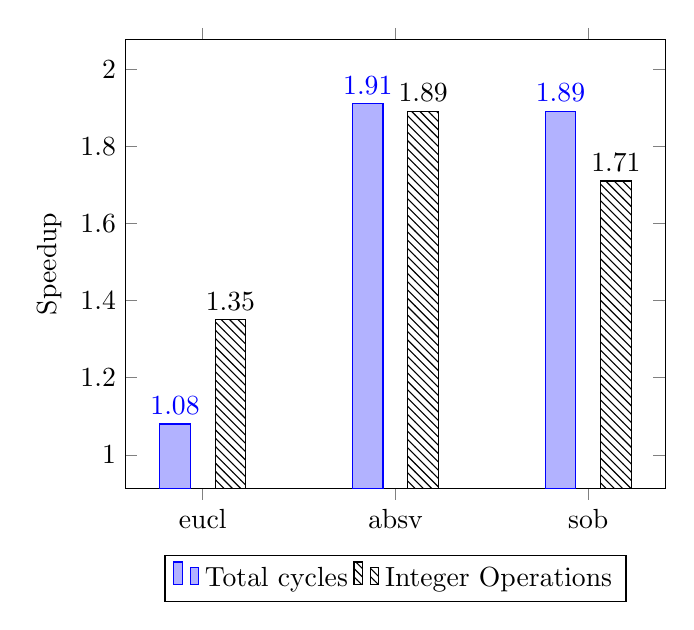
\begin{tikzpicture}
\begin{axis}[
    ybar,
    enlargelimits=0.2,
    legend style={at={(0.5,-0.15)},
    anchor=north,legend columns=-1},
    ybar=9pt,% configures `bar shift'
    bar width=11pt,
    ylabel={Speedup},
    symbolic x coords={eucl,absv,sob},
    xtick=data,
    nodes near coords,
    nodes near coords align={vertical},
    ]
\addplot coordinates {(eucl,1.08) (absv,1.91) (sob,1.89)};
\addplot[postaction={pattern=north west lines}] coordinates {(eucl,1.35) (absv,1.89) (sob,1.71)};
\legend{Total cycles,Integer Operations}
\end{axis}
\end{tikzpicture}}
\caption{Cycles comparison.} 
\label{fig:cycles}
\end{figure}


The \emph{eucl} instruction got the smaller reduction because its transformation only combined two separated assembly instructions (substract and then multiply)
into one operation. The \emph{sob} instruction, although somewhat similar to the \emph{eucl}, got a bigger reduction in number of cycles because it transformed
tree single assembly operations (two multiplications and one addition) into only one special instruction. Finally, the \emph{absv} got the most significant reduction
in total cycles since it performs a very specific operation, while the normal assembly instructions' version used branch logic to test for a negative value in the substraction
and apply the proper operation.


The additional area caused by the ASIP hardware had a minimal impact compared to the general processor, as showed in Table \ref{tab:area}.
Every optimized version of the processor for each special instruction had a difference of area of 1\% at most compared to the processor without the ASIP,
which for practical use is not significant. 



\begin{table}[t!]
\begin{center}
\caption{Area comparison}
\resizebox{0.5\textwidth}{!}{\begin{tabular}{|c|c|c|c|c|} 
 \hline
Metric	&\emph{eucl} instr.	&\emph{absv} instr.	&\emph{sob} instr.	&No special instr. \\  \hline
\# Slices	&3998	&4058	&4223	&3990 \\ \hline
\% Slices	&5\%	&5\%	&6\%	&5\% \\ \hline
\# LUTs	&6384	&6465	&6079	&6199 \\ \hline
\% LUTs	&9\%	&9\%	&8\%	&8\% \\ \hline
 \end{tabular}}
\label{tab:area}
\end{center}
\end{table}



As same as the area, the impact on the power was very low, as showed in Figures \ref{fig:dynaPower} and \ref{fig:power}.
The maximum difference on power was 5 mW in the dynamic power, as showed in Figure \ref{fig:dynaPower}. 
The quiescent power stayed the same for all processor's versions, at 1163 mW, which added to the dynamic
power makes a total power between 1493 to 1498 mW; as showed in Figure \ref{fig:power} this difference
is not noticeable.

\begin{figure}[t!]
\centering
\resizebox{0.5\textwidth}{!}{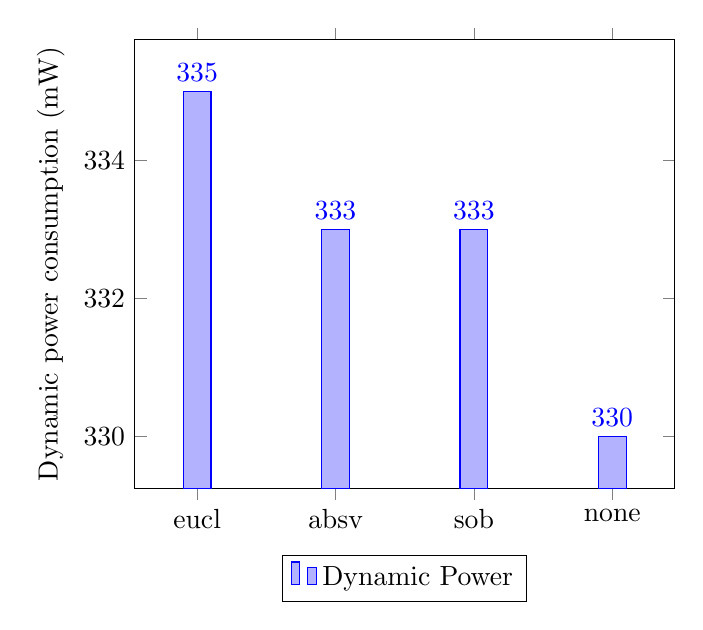
\begin{tikzpicture}
\begin{axis}[
    ybar,
    enlargelimits=0.15,
    legend style={at={(0.5,-0.15)},
    anchor=north,legend columns=-1},
    ylabel={Dynamic power consumption (mW)},
    symbolic x coords={eucl,absv,sob, none},
    xtick=data,
    nodes near coords,
    nodes near coords align={vertical},
    ]
\addplot coordinates {(eucl,335) (absv,333) (sob,333) (none,330)};
\legend{Dynamic Power}
\end{axis}
\end{tikzpicture}}
\caption{Cycles comparison.} 
\label{fig:dynaPower}
\end{figure}


\begin{figure}[t!]
\centering
\resizebox{0.5\textwidth}{!}{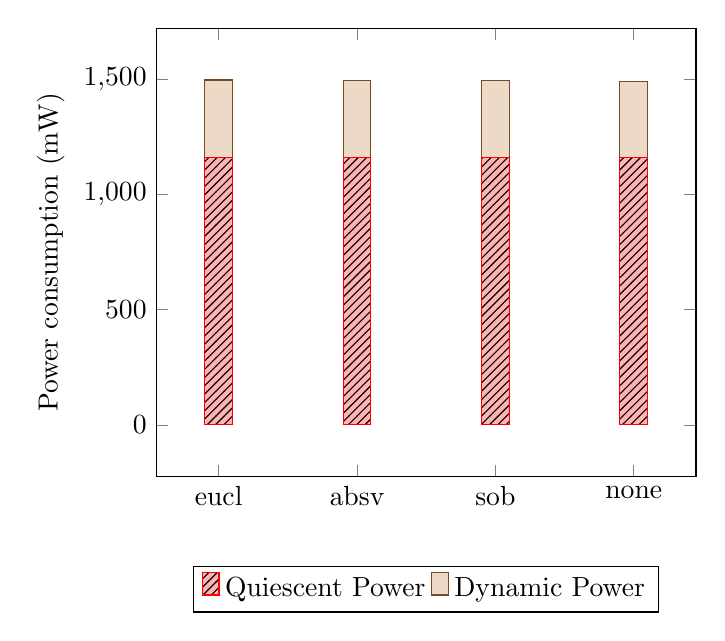
\begin{tikzpicture}
\begin{axis}[
    ybar stacked,
    enlargelimits=0.15,
    legend style={at={(0.5,-0.20)},
      anchor=north,legend columns=-1},
    ylabel={Power consumption (mW)},
    symbolic x coords={eucl, absv, sob, none},
    xtick=data,
    ]
\addplot+[ybar] plot coordinates {(eucl,0) (absv,0) 
  (sob,0) (none,0)};
\addplot+[ybar,postaction={pattern=north east lines}] plot coordinates {(eucl,1163) (absv,1163) 
  (sob,1163) (none,1163)};
\addplot+[ybar] plot coordinates {(eucl,335) (absv,333) 
  (sob,333) (none,330)};
\legend{, Quiescent Power, Dynamic Power}
\end{axis}
\end{tikzpicture}}
\caption{Power comparison.} 
\label{fig:power}
\end{figure}


The minimum impact on area and power was mainly due to the main processor having already a lot of hardware
to support common assembly instructions, and while almost the whole processor remained, for all the three special instructions,
the same for flexibility purposes, a considerable reduction in execution time was achieved. 

\section{Conclusion}


The developed ASIPs showed speedups in total of cycles of almost 2X while increasing the overall hardware area and power at roughly  1\% and 5mW respectively compared to the unmodified version.
Future work involves implementing hardware-level approximation for the SI logic developed, which will increase the execution time at a cost of output quality, which 
will further give the ASIPs the freedom to adjust to more type of needs in different scenarios.



\bibliographystyle{sty/plainurl}
\bibliography{references}




% that's all folks
\end{document}


